% !TeX spellcheck = en_GB

\section{Online Analytic Processing (OLAP)}

\begin{breakbox}
\boxtitle{OLAP Operations}
\newline Slice-and-dice:
\begin{center}
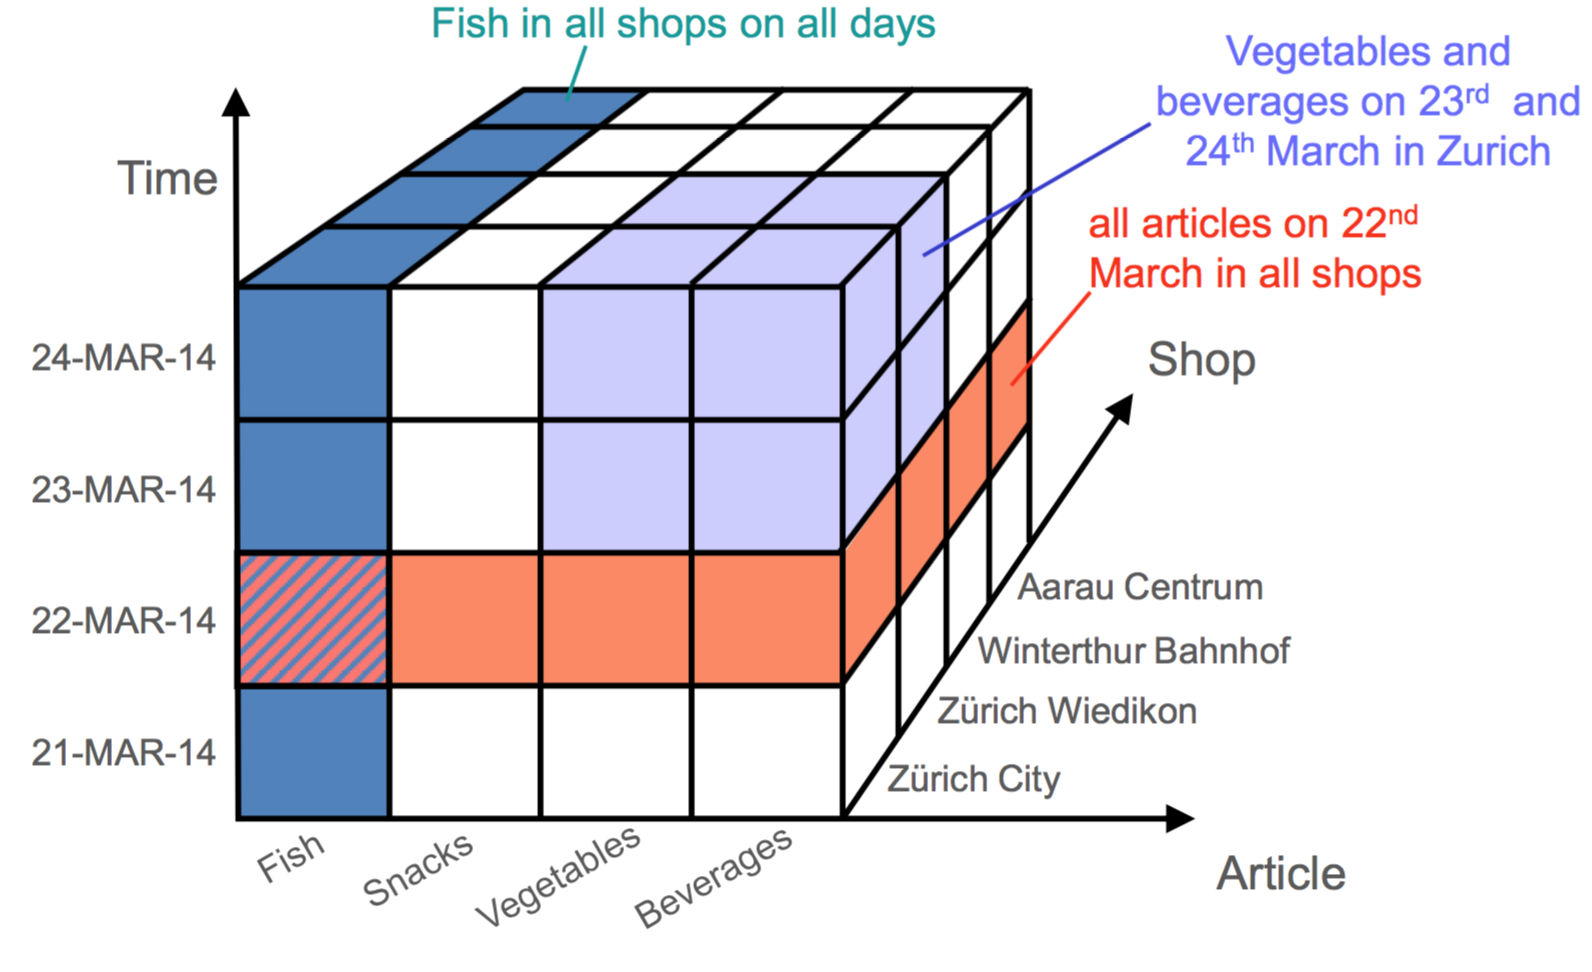
\includegraphics[width=.1\textwidth]{slides_images/slice_and_dice}
\end{center}
Drill-down:
\begin{center}
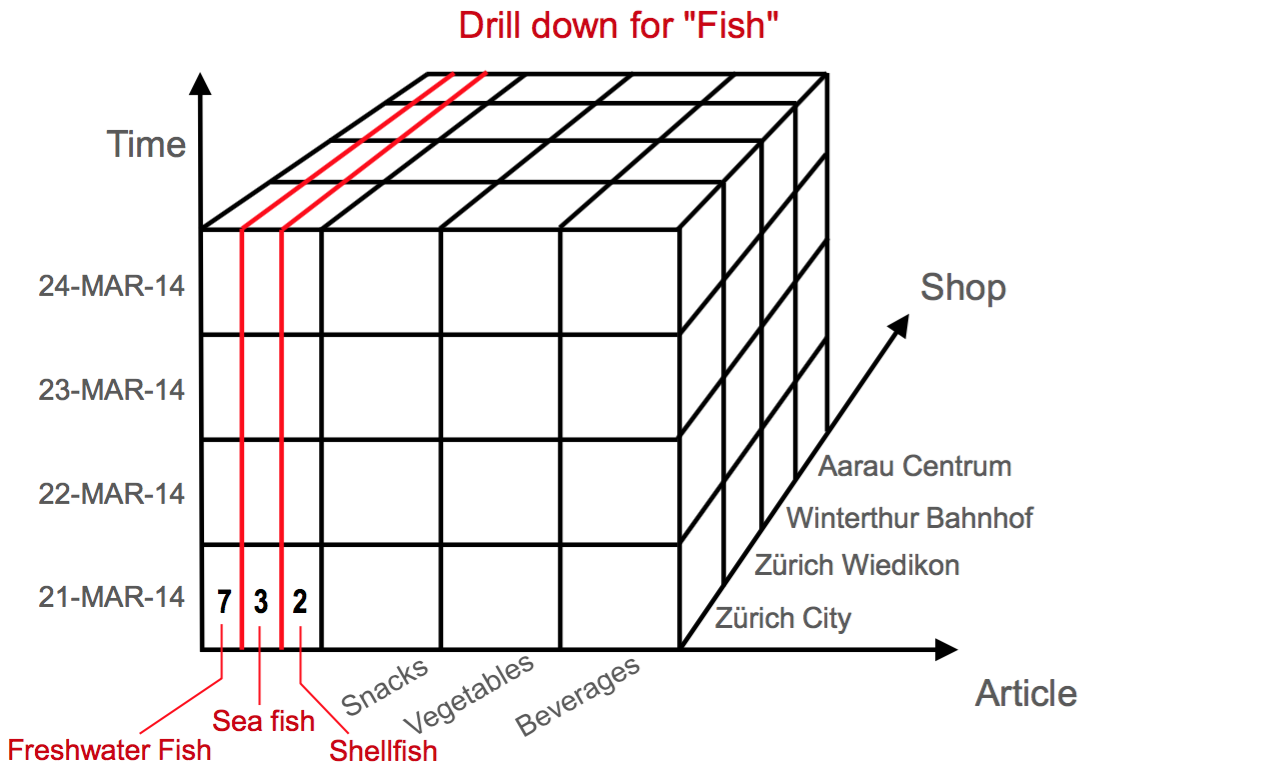
\includegraphics[width=.1\textwidth]{slides_images/drill_down}
\end{center}
Roll-up:
\begin{center}
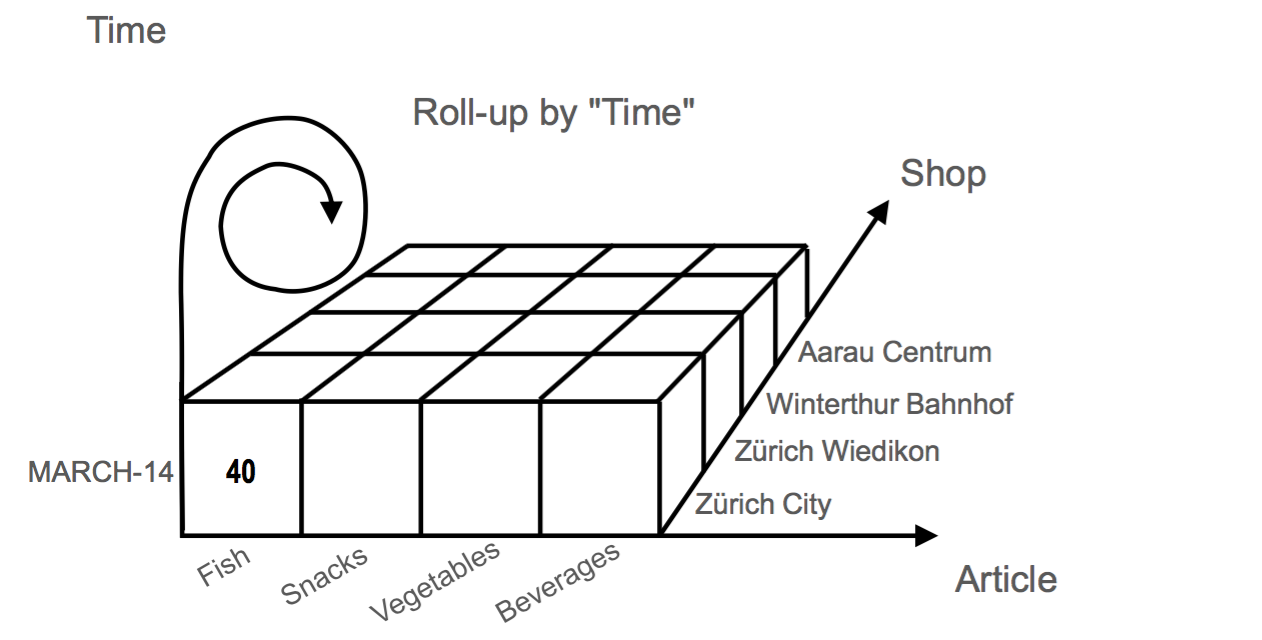
\includegraphics[width=.1\textwidth]{slides_images/roll_up}
\end{center}
\end{breakbox}

\begin{breakbox}
\boxtitle{ROLLUP:}
\sql{sql_code/rollup.sql}
Dimensions are grouped from left to right.
\end{breakbox}

\begin{breakbox}
\boxtitle{CUBE:}
Does every possible \lstinline{ROLLUP}.
\sql{sql_code/cube.sql}
Note:
\begin{itemize}
	\item Cube has $2^n$ entries for n dimensions.
	\item Result of the CUBE Operator contains all entries to build cross tabulations:
\end{itemize}
\begin{center}
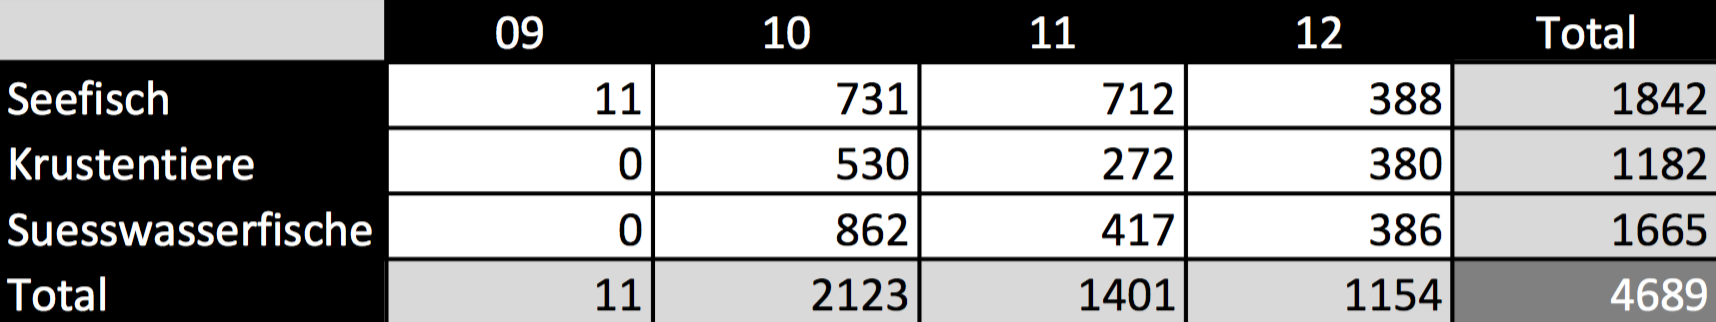
\includegraphics[width=.15\textwidth]{slides_images/cross_tabulation}
\end{center}
\end{breakbox}

\begin{breakbox}
\boxtitle{Bi-Temporal Tables:}
\newline Update:
\begin{center}
	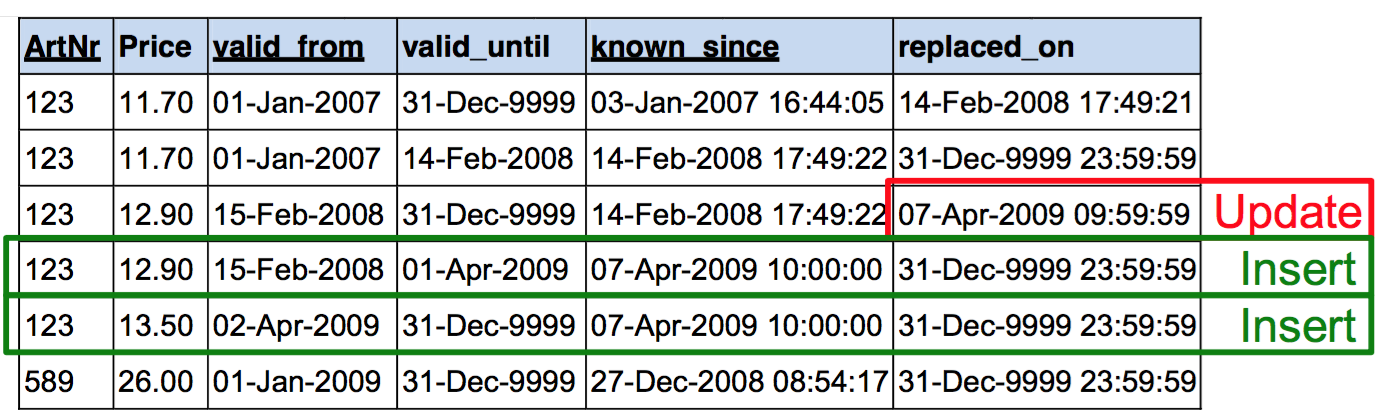
\includegraphics[width=.15\textwidth]{slides_images/bi_temporal_update}
\end{center}
Note:
\begin{itemize}
	\item The valid\_from and the known\_since entries are combined with ArtNr to build the new primary key.
\end{itemize}
\end{breakbox}
%\begin{breakbox}
%\boxtitle{CREATE Star Schema:}
%\sql{sql_code/create_star_schema.sql}
%\end{breakbox}
